% !TeX spellcheck = en_GB
% !TeX program = pdflatex
%
% LuxSleek-CV 1.1 LaTeX template
% Author: Andreï V. Kostyrka, University of Luxembourg
%
% 1.1: added tracking and letter-spacing for prettier lower caps, added `~` for language levels
% 1.0: initial release
%
% This template fills the gap in the available variety of templates
% by proposing something that is not a custom class, not using any
% hard-coded settings deeply hidden in style files, and provides
% a handful of custom command definitions that are as transparent as it gets.
% Developed at the University of Luxembourg.
%
% *NOTHING IS HARCODED, and never should be.*
%
% Target audience: applicants in the IT industry, or business in general
%
% The main strength of this template is, it explicitly showcases how
% to break the flow of text to achieve the most flexible right alignment
% of dates for multiple configurations.

\documentclass[11pt, a4paper]{article} 

\usepackage[T1]{fontenc}     % We are using pdfLaTeX,
\usepackage[utf8]{inputenc}  % hence this preparation
\usepackage[british]{babel}  
\usepackage[left = 0mm, right = 0mm, top = 0mm, bottom = 0mm]{geometry}
\usepackage[stretch = 25, shrink = 25, tracking=true, letterspace=30]{microtype}  
\usepackage{graphicx}        % To insert pictures
\usepackage{xcolor}          % To add colour to the document
\usepackage{marvosym}        % Provides icons for the contact details

\usepackage{enumitem}        % To redefine spacing in lists
\setlist{parsep = 0pt, topsep = 0pt, partopsep = 1pt, itemsep = 1pt, leftmargin = 6mm}

\usepackage{FiraSans}        % Change this to use any font, but keep it simple
\renewcommand{\familydefault}{\sfdefault}

\definecolor{cvblue}{HTML}{304263}

%%%%%%% USER COMMAND DEFINITIONS %%%%%%%%%%%%%%%%%%%%%%%%%%%
% These are the real workhorses of this template
\newcommand{\dates}[1]{\hfill\mbox{\textbf{#1}}} % Bold stuff that doesn’t got broken into lines
\newcommand{\is}{\par\vskip.5ex plus .4ex} % Item spacing
\newcommand{\smaller}[1]{{\small$\diamond$\ #1}}
\newcommand{\headleft}[1]{\vspace*{3ex}\textsc{\textbf{#1}}\par%
    \vspace*{-1.5ex}\hrulefill\par\vspace*{0.7ex}}
\newcommand{\headright}[1]{\vspace*{2.5ex}\textsc{\Large\color{cvblue}#1}\par%
     \vspace*{-2ex}{\color{cvblue}\hrulefill}\par}
%%%%%%%%%%%%%%%%%%%%%%%%%%%%%%%%%%%%%%%%%%%%%%%%%%%%%%%%%%%%

\usepackage[colorlinks = true, urlcolor = white, linkcolor = white]{hyperref}

\begin{document}

% Style definitions -- killing the unnecessary space and adding the skips explicitly
\setlength{\topskip}{0pt}
\setlength{\parindent}{0pt}
\setlength{\parskip}{0pt}
\setlength{\fboxsep}{0pt}
\pagestyle{empty}
\raggedbottom

\begin{minipage}[t]{0.33\textwidth} %% Left column -- outer definition
%  Left column -- top dark rectangle
\colorbox{cvblue}{\begin{minipage}[t][5mm][t]{\textwidth}\null\hfill\null\end{minipage}}

\vspace{-.2ex} % Eliminates the small gap
\colorbox{cvblue!90}{\color{white}  %% LEFT BOX
\kern0.09\textwidth\relax% Left margin provided explicitly
\begin{minipage}[t][293mm][t]{0.82\textwidth}
\raggedright
\vspace*{2.5ex}

\Large John \textbf{\textsc{Miller}} \normalsize 

% Centering without extra vertical spacing
\null\hfill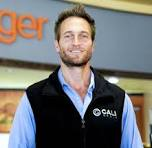
\includegraphics[width=0.65\textwidth]{joh.png.jpg}\hfill\null

\vspace*{0.5ex} % Extra space after the picture

\headleft{Profile Summary}
Experienced \textit{Data Analyst} with over 5+ years of expertise in SQL,Python, Excel, Power BI, Power BI Service, T-SQL, Birt Reporting tool, and Kibana. Proficient in data manipulation, statistical analysis, and data visualization. Skilled in data collection, cleansing, analysis, and creating insightful visual reports to support data-driven decision-making. Strong communicator with a track record of translating complex data into actionable business insights.

\headleft{Contact details}
\small % To fit more content
\MVAt\ {\small XXXXXXX@gmail.com} \\[0.4ex]
\Mobilefone\ +91\,00\,00\,00\,00\,00 \\[0.5ex]
\Letter\ XXXXXXXXXXXXX
\normalsize

\headleft{Personal information}
%Year of birth: \textbf{1861} \\[0.5ex]
Citizenship: \textbf{Indian} \\[0.5ex]
Family: \textbf{Married with children} \\[0.5ex]
Languages: \textbf{English}, \textbf{Hindi}, \textbf{Telugu}

\headleft{Skills}
\begin{itemize}
\item SQL, SSMS, Power BI,Power BI Service, DAX Functions,
Tableau, Python, PySpark
\item Panda, Numpy, Warehouse, Azure Databricks
\item Microsoft Excel, MS Word,MS PowerPoint
\item SQL Server, T-SQL, Kibana,Eclipse Birt,ETL
\item JavaScript, HTML, GitHub
\item Communication and team collaboration
\end{itemize} 

\end{minipage}%
\kern0.09\textwidth\relax%%Right margin provided explicitly to stretch the colourbox
}
\end{minipage}% Right column
\hskip2.5em% Left margin for the white area
\begin{minipage}[t]{0.56\textwidth}
\setlength{\parskip}{0.8ex}% Adds spaces between paragraphs; use \\ to add new lines without this space. Shrink this amount to fit more data vertically

\vspace{2ex}

\headright{Experience}

\textsc{Data analyst} at \textit{XXXX (Hyderabad).}  \dates{2018.08--2024.05} \\

\smaller{Collected, cleaned, and processed large datasets from multiple sources to ensure data accuracy and integrity.}

\is
\smaller{Conducted exploratory data analysis to identify patterns, trends, and insights using statistical methods and data visualization techniques to support business decisions.}

\is
\smaller{Maintained automated data pipelines for efficient data extraction, transformation, and loading (ETL) processes using SQL and Python}

\is
\smaller{Created interactive dashboards and reports using Power BI, DAX Function and Power BI Service to visualize key performance indicators (KPIs) and communicate findings to stakeholders}

\is
\smaller{Collaborated with cross-functional teams to define project requirements, analyze business problems, and develop data-driven solutions. Conducting ad-hoc analysis and insights to support strategic initiatives and business objectives.}

\is 
\smaller{Conducted data quality assessments and implemented data governance policies to ensure data accuracy, consistency, and compliance.}

\is
\smaller{Create complex SQL queries using UNION and UNION ALL, Join’s, GROUP BY, WHERE, and HAVING conditions for report and dashboard creation. Optimize SQL queries and create stored procedures, views, functions, and indexes. Created temp tables, CTEs, and variables for data manipulation.} 

\is
\smaller{Having good experience on T-SQL, Microsoft SQL Server
Management Studio. Solid knowledge of database management systems and data warehousing concepts.}

\is
\smaller{Having good knowledge creating Relationships in data model like one-one, one-many, many-one and many-many. Monitoring and validating key metrics insights data from daily report.}

\headright{Education}

\textsc{Master of Computer Application (MCA).} \textit{from JNTU Kakinada University}. \dates{2012--2015} \\

\is
\textsc{Bachelor of Science in Mathematics, Physics, and Computer
Science.} \textit{Acharya Nagarjuna University}.  \dates{2007--2010} \\

\headright{Certifications}

\smaller{\textsc{Introduction to Data Analysis using Microsoft Excel,}} \textit{Coursera.} \\
\is
\smaller{\textsc{Data Analysis With Python,Cognitive Class DA0101EN,} \textit{provided by IBM.}} \dates{July-3-2024} \\
\is
\smaller{\textsc{SQL, Hacker Rank}}

\headright{Hobbies}

\textit{Listening Music, Playing Cricket}
\end{minipage}

\end{document}
